%%%%%%%%%%%%%%%%%%%%%%%%%%%%%%%%%%%%%%%%%%%%%%%%%%%%%%%%%%%%%%%%%%%%%%
% How to use writeLaTeX: 
%
% You edit the source code here on the left, and the preview on the
% right shows you the result within a few seconds.
%
% Bookmark this page and share the URL with your co-authors. They can
% edit at the same time!
%
% You can upload figures, bibliographies, custom classes and
% styles using the files menu.
%
%%%%%%%%%%%%%%%%%%%%%%%%%%%%%%%%%%%%%%%%%%%%%%%%%%%%%%%%%%%%%%%%%%%%%%

\documentclass[12pt]{article}

\usepackage{sbc-template}

\usepackage{graphicx,url}

\usepackage[brazil]{babel}   
\usepackage[utf8]{inputenc}  

     
\sloppy

\title{Análise de Desempenho Paralelo de Modelos de Difusão de Contaminantes em Água}

\author{Eduardo Verissimo Faccio, Pedro Figueiredo Dias, \\
Pedro Henrique de Oliveira Masteguin}


\address{Instituto de Ciência e Tecnologia -- Universidade Federal de São Paulo (UNIFESP)\\
    São José dos Campos -- SP -- Brasil
  \email{\{verissimo.eduardo,pedro.figueiredo,p.masteguin\}@unifesp.br}
}

\begin{document} 

\maketitle
     
% \begin{resumo} 
%   Este meta-artigo descreve o estilo a ser usado na confecção de artigos e
%   resumos de artigos para publicação nos anais das conferências organizadas
%   pela SBC. É solicitada a escrita de resumo e abstract apenas para os artigos
%   escritos em português. Artigos em inglês deverão apresentar apenas abstract.
%   Nos dois casos, o autor deve tomar cuidado para que o resumo (e o abstract)
%   não ultrapassem 10 linhas cada, sendo que ambos devem estar na primeira
%   página do artigo.
% \end{resumo}

\section{Introdução}


\section{Implementação do Algorítimo}

\subsection{Código Sequencial}

O código sequencial implementa a solução numérica da equação de difusão usando uma abordagem serial. Utilizando-se do método de diferenças finitas, é simulado a dispersão de uma substância em uma matriz bidimensional. Cada célula da matriz representa a concentração de uma substância em um ponto do espaço.

O cálculo é realizado em um laço de repetição que itera sobre todas as células da matriz. A atualização de cada célula depende da média das concentrações dos seus vizinhos imediatos e de parâmetros físicos como coeficiente de difusão, o intervalo de tempo \textit{dt} e o espaçamento espacial \textit{dx}.

\subsection{Código Paralelo}

O código paralelo implementa uma versão desenvolvida em OpenMP do mesmo algorítimo sequencial, para distribuir o trabalho entre múltiplos núcleos do processador. Isso é alcançado utilizando-se das diretivas específicas da biblioteca na estrutura do código sequencial.

\begin{itemize}
    \item \#pragma omp parallel for collapse(2): É a diretiva que divide automaticamente os loops de cálculo entre múltiplos threads. Cada thread é responsável por atualizar uma parte distinta da matriz, permitindo que várias partes do cálculo sejam realizadas simultaneamente. O uso de collapse(2) indica que o compilador deve tratar múltiplas laços aninhados com um único para fins de paralelismo. No caso do código de difusão, os dois laços de repetição aninhados serão linearizados.
    \item \#pragma omp parallel for reduction(+:difmedio) collapse(2): Essa diretiva assim como a anterior executa as iterações do laço de repetição de maneira paralela, com o adicional de reduções, que garantem que a operação de somatório que monitora a convergência do algorítimo seja realizada de maneira segura entre as diferentes threads que acessam as variáveis dessa operação.
    \item omp\_set\_num\_threads(int num\_threads): Permite configurar dinamicamente o número de threads a serem utilizados pelo código, sendo extremamente útil para realizar as verificações de desempenho.
\end{itemize}

\subsection{Interface Python e ferramenta CMake}

O projeto utiliza o CMake como sistema de compilação, definindo processos e dependências (como a biblioteca OpenMP) por meio de um arquivo de configuração. Para evidenciar as diferenças de desempenho entre as implementações sequencial e paralela, desativamos otimizações do compilador usando flags específicas, pois otimizações como a vetorização automática no código sequencial reduziram inicialmente essa diferença. Assim, desabilitar essas otimizações permitiu uma execução mais direta, destacando as diferenças de desempenho entre as abordagens.

Além disso, implementamos uma interface Python usando o módulo ctypes para carregar a biblioteca de difusão em C e mapear suas funções e, com isso, permite executar os códigos sequencial e paralelo de forma flexível, facilitando a integração com métodos de análise desenvolvidos em notebooks Jupyter, onde os resultados são visualizados. Criar essa interface segue a abordagem de outras grandes bibliotecas da linguagem, combinando a facilidade de uso de um ambiente de alto nível com a eficiência de soluções implementadas em linguagens como C. Um exemplo de biblioteca que utiliza esse método é o NumPy, que oferece operações matemáticas de alto desempenho por meio de códigos otimizados em C.

\section{Resultados}

Nesta seção, apresentamos os resultados obtidos de nossa implementação. Inicialmente, analisamos a equivalência lógica entre os códigos sequencial e paralelo, considerando possíveis erros que podem surgir na paralelização, como condições de corrida ou inconsistências de sincronização. Em seguida, ilustramos, por meio de mapas de calor, a atualização dos valores da matriz ao longo do tempo. Por fim, realizamos uma análise comparativa dos tempos médios de execução, \textit{speedup} e eficiência entre as duas versões.

\subsection{Validação da Implementação}

Para assegurar a correção das duas implementações, verificamos em cada iteração se os valores presentes em cada célula da matriz são idênticos. Dessa forma, o resultado na última iteração deve ser o mesmo em ambas as versões.

Por meio desse procedimento, utilizando a interface Python em conjunto com um Jupyter Notebook, comprovamos que as duas soluções produzem resultados idênticos. Isso era esperado, pois no código paralelo não ocorrem condições de corrida, uma vez que a escrita não é realizada na mesma região de memória das leituras, tornando o processamento de cada célula pelas \textit{threads} independente.

\subsection{Validação da Implementação}

Para ilustrar o funcionamento da implementação, foram gerados mapas de calor, representado pela Figura \ref{fig:heatmap}, nos quais cada ponto de uma matriz 50x50 é representado por uma cor distinta. Cores escuras correspondem a valores próximos de um, indicando alta concentração do contaminante, enquanto cores claras representam valores próximos de zero, indicando baixa presença de contaminação.

\begin{figure}[ht]
\centering
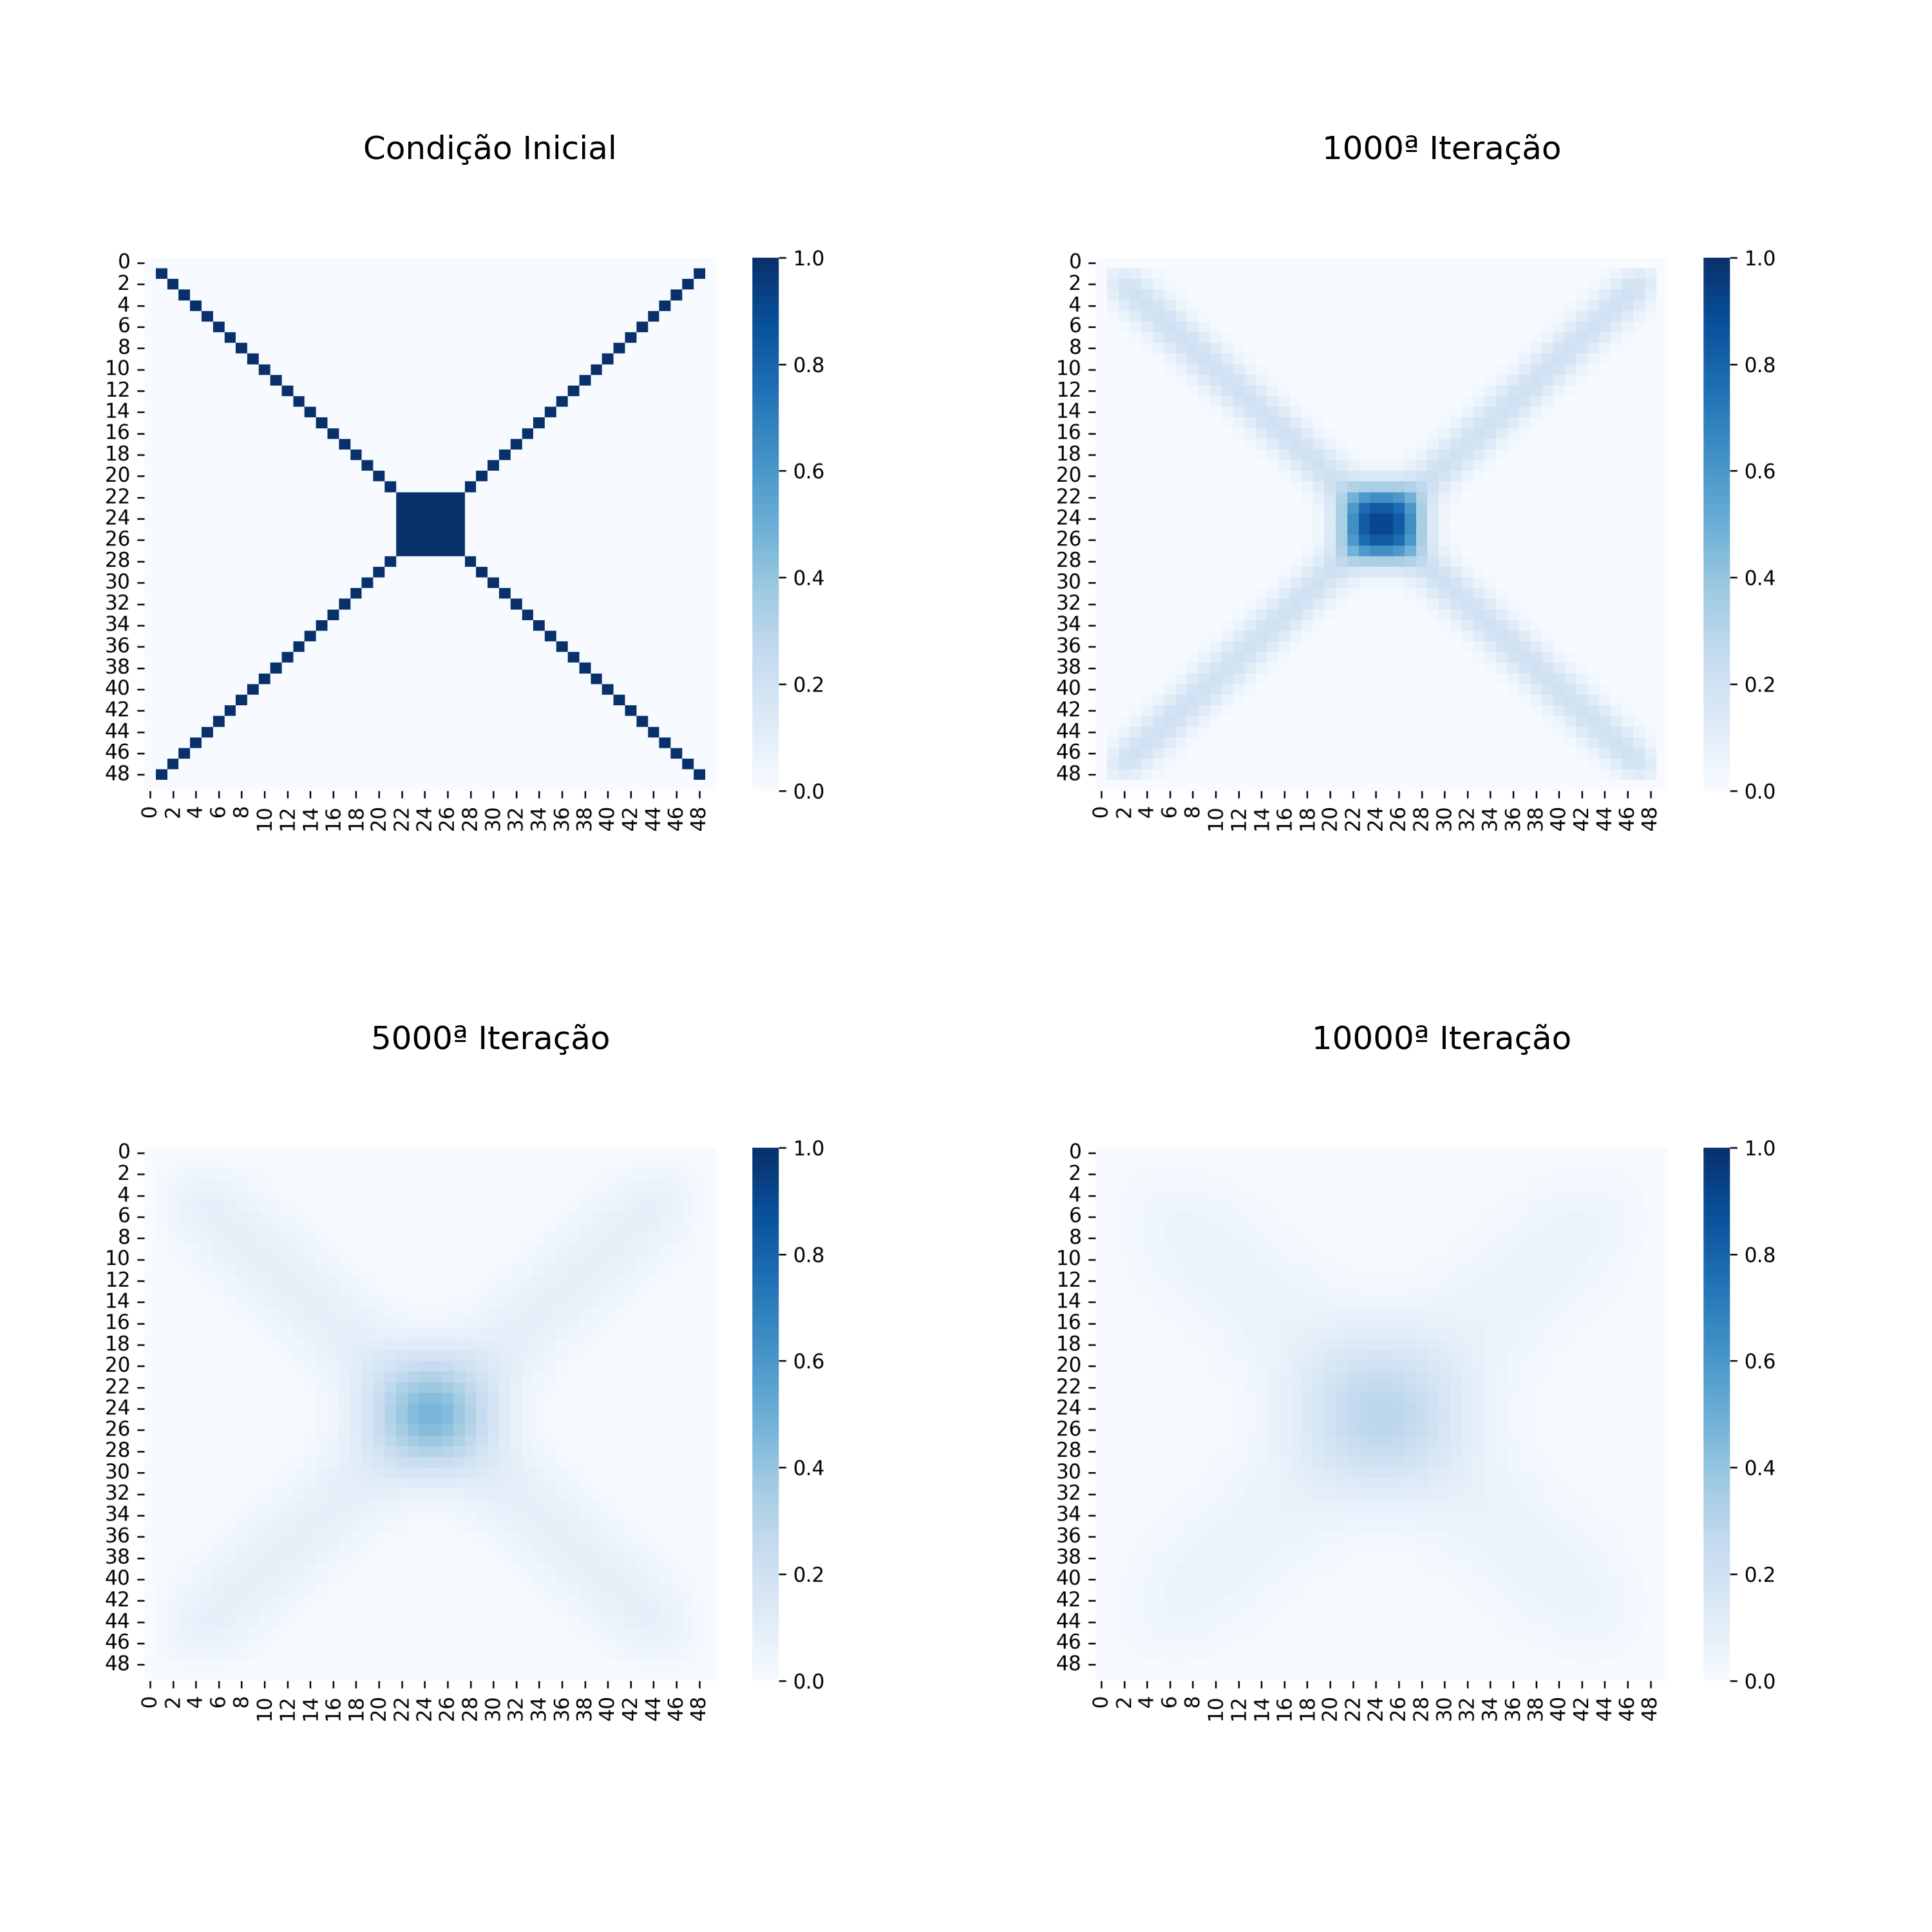
\includegraphics[width=.7\textwidth]{figs/heatmap.png}
\caption{Mapa de calor em quatro instantes distintos da simulação.}
\label{fig:heatmap}
\end{figure}

Analisando a progressão dos mapas de calor, observamos que o comportamento faz sentido no contexto da solução proposta. Inicialmente, o contaminante é adicionado com alta concentração nas diagonais e no centro da matriz, evidenciado pelas regiões azuis escuros. Com o avanço das iterações, o contaminante começa a se difundir para as regiões adjacentes, aumentando gradativamente a luminosidade nessas áreas e diminuindo nos pontos de concentração inicial. Na última iteração, a concentração se distribui uniformemente pela matriz, com valores próximos entre si.

\subsection{Análise de Desempenho}

A análise de desempenho foi realizada em um computador \textit{desktop} com as seguintes especificações. Além disso, as especificações dos parâmetros do problema foram incluídas na tabela correspondente.

\begin{table}[ht]
\centering
\caption{Tabela de especificação de Hardware}
\vspace{0.3cm}
\begin{tabular}{||c c||} 
 \hline
Especificações & Detalhes \\ [0.5ex] 
 \hline\hline
 Processador & Intel i7-4790 @ 3.60GHz \\ 
 \hline
 Núcleos / Lógicos & 4 / 8  \\
 \hline
 Memória RAM & 8 GB  \\
 \hline
 Sistema Operacional & Ubuntu 22.04.05 (via WSL)   \\ 
 \hline
\end{tabular}
\end{table}

\begin{table}[ht]
\centering
\caption{Tabela de especificação da Simulação}
\vspace{0.3cm}
\begin{tabular}{||c c||} 
 \hline
Especificações & Detalhes \\ [0.5ex] 
 \hline\hline
 Dimensão da Matriz (N x N) & 2000 x 2000 \\ 
 \hline
 Número de Iterações & 500  \\
 \hline
 Distribuição Inicial & Alta concentração no centro  \\
 \hline
 Coeficiente de Difusão & 0.1   \\ 
 \hline
 dt & 0.01   \\ 
 \hline
 dx & 1.0   \\ 
 \hline
\end{tabular}
\end{table}

Para obter valores mais consistentes e minimizar influências externas, como outros programas em execução, cada teste foi executado quinze vezes e, assim, calculamos o tempo médio gasto e seu desvio padrão. O \textit{speedup} é calculado dividindo-se o tempo de execução sequencial pelo tempo de execução paralelo correspondente, enquanto a eficiência é determinada ao dividir o \textit{speedup} pelo número de \textit{threads} utilizados.

\begin{table}[ht]
\centering
\caption{Tabela de comparação de desempenho entre o código sequencial e o paralelo utilizando OpenMP.}
\vspace{0.3cm}
\begin{tabular}{||c c c c||} 
 \hline
 Nº Threads & Tempo & Speedup & Eficiência \\ [0.5ex] 
 \hline\hline
 1 & 26.22 $\pm$ 2.09 & 1.0 & 100\% \\ 
 \hline
 2 & 14.59 $\pm$ 1.49 & 1.80 & 89,88\% \\
 \hline
 4 & 10.60 $\pm$ 1.43 & 2.47 & 61.82\% \\
 \hline
 8 & 8.52 $\pm$ 1.32 & 3.08 & 38.48\% \\
 \hline
 16 & 8.29 $\pm$ 1.29 & 3.16 & 19.77\% \\
 \hline
 32 & 8.67 $\pm$ 1.43 & 3.03 & 9.45\% \\ 
 \hline
\end{tabular}
\end{table}

\begin{figure}[ht]
\centering
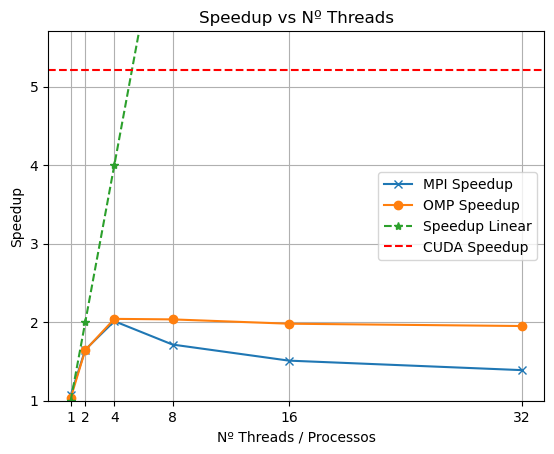
\includegraphics[width=.5\textwidth]{figs/speedupxthreads.png}
\caption{Gráfico do \textit{speedup} por número de \textit{threads}}
\label{fig:speedupOMP}
\end{figure}

\begin{figure}[ht]
\centering
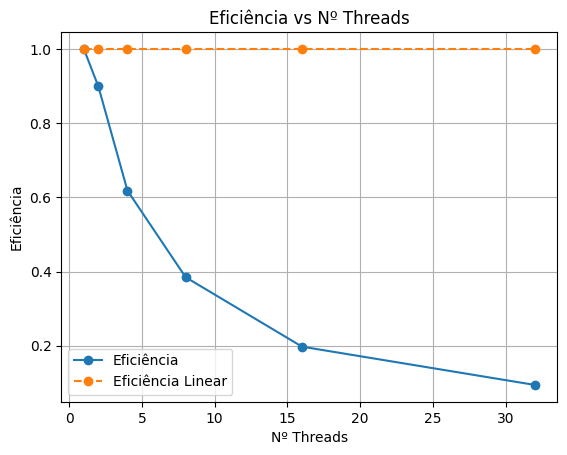
\includegraphics[width=.5\textwidth]{figs/eficienciaxthreads.png}
\caption{Gráfico da eficiência por número de \textit{threads}}
\label{fig:eficienciaOMP}
\end{figure}


O gráfico de \textit{speedup} (Figura \ref{fig:speedupOMP}) mostra uma tendência de estabilização em torno do valor três, enquanto o \textit{speedup} linear ideal apresenta valores significativamente maiores, o que pode sugerir que a escalabilidade da aplicação é limitada, possivelmente devido a \textit{overheads} de sincronização ou ao fato de que o problema não é suficientemente grande para aproveitar eficientemente um número maior de \textit{threads}. Além disso, o desempenho pode estar sendo afetado pela latência de memória ou pela arquitetura do processador utilizado e, consequentemente, não há grandes vantagens em utilizar um número elevado de \textit{threads} para resolver este problema específico.

\section{Conclusão}
Por meio de implementações sequenciais e paralelas utilizando OpenMP, foi validada a correção dos resultados e analisou-se o impacto do paralelismo no tempo de execução. Os resultados obtidos mostraram que, embora o paralelismo traga ganhos significativos em relação ao código sequencial, há limitações na escalabilidade, possivelmente devido a fatores como \textit{overheads} de sincronização e restrições arquiteturais do hardware utilizado. Assim, este trabalho reforça os conceitos fundamentais aprendidos em programação concorrente e distribuída, evidenciando as vantagens práticas da paralelização em termos de desempenho e eficiência em simulações numéricas.

\section{References}



\bibliographystyle{sbc}
\bibliography{sbc-template}

\end{document}
